\chapter{Razvojni sustav STM32WB5MM-DK}

Razvojni sustav temelji se na modulu STM32WB5MMG tvrtke \textit{STMicroelectronics}, koji je dio linije STM32WBx5 razvojnih sustava. Kao i svi mikrokontroleri iz te skupine, modul sadrži 32-bitni aplikacijski procesor ARM Cortex-M4 koji radi na frekvenciji do 64 MHz te mrežni procesor Cortex-M0+ s frekvencijom rada do 32MHz. Modul sadrži 1 MB memorije tipa \textit{Flash} i 256 KB memorije tipa SRAM (engl. \textit{Static random-access memory}).\cite{stm32manual} Budući da modul ima funkciju RF (engl. \textit{radio frequency}) primopredajnika, podržava protokole Bluetooth, Zigbee, Thread i konkurentne bežične standarde. Sustav također ima 0.96-inčni 128x64 zaslon, RGB LED diode te senzore za temperaturu, dodir, \textit{Time-of-Flight} senzor i žiroskop. Od ostale periferije najznačajniji je digitalni MEMS mikrofon. Modul STM32WB5MMG je višeprotokolni, bežični uređaj niske potrošnje energije (engl. \textit{ultra-low-power}) primarno namijenjen razvoju aplikacija koje koriste audio, USB ili \textit{Bluetooth Low Energy} (BLE) protokol. 

\begin{figure}[ht]
	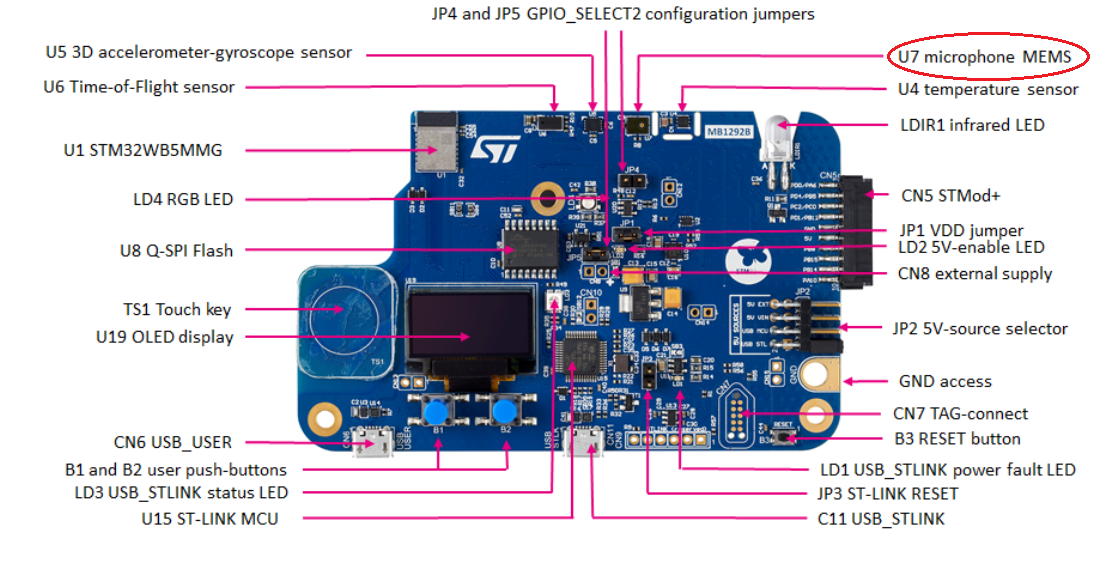
\includegraphics[width=\linewidth]{imgs/discovery_kit}
	\caption{Konfiguracija razvojnog sustava STM32WB5MM-DK \cite{stm32manual}}
	\label{fig:discovery-kit}
\end{figure}

\section{BLE protokol}

Bluetooth protokol korišten je za povezivanje razvojnog sustava s matičnim računalom i za prijenos audio signala s mikrokontrolera. BLE je vrsta bežične komunikacije namijenjena komunikaciji kratkog dometa s niskom potrošnjom energije. Razvijen je kako bi se postigao standard vrlo male snage koji radi s baterijom veličine kovanice (engl. \textit{coin-cell batteries}) nekoliko godina.
Klasična Bluetooth tehnologija razvijena je kao bežični standard, što je omogućilo razvoj bežičnih i prenosivih uređaja, no ne podržava dug život baterije zbog brze i nepredvidive komunikacije te složenih postupaka povezivanja. BLE uređaji troše samo dio energije koju troše standardni Bluetooth proizvodi te omogućavaju malenim uređajima s malim baterijama bežično povezivanje s uređajima koji koriste klasični Bluetooth. \cite{blevsbluetooth}

BLE radi u istom opsegu od 2,4 GHz kao i standardni Bluetooth, no koristi različite kanale od standardnog Bluetootha. Koristi 40 kanala od 2 MHz za prijenos podataka korištenjem modulacije Gaussova pomaka frekvencije (metoda koja se koristi za glatkije prijelaze između podatkovnih impulsa), zbog čega skokovi frekvencije proizvode manje smetnji u usporedbi sa standardnom Bluetooth komunikacijom.

Arhitektura BLE tehnologije naziva se još i BLE stog zbog slojevite strukture. Stog se sastoji od dvije glavne komponente:
\begin{itemize}
	\item upravljač (engl. \textit{controller}),
	\item domaćin (engl. \textit{host}).
\end{itemize}

Upravljač se sastoji od fizičkog sloja i sloja veze. Host uključuje protokol kontrole i prilagodbe logičke veze (\textit{Logical Link Control and Adaptation Layer Protocol} - L2CAP), upravitelja sigurnosti (\textit{Security Manager} - SM), protokol atributa (\textit{Attribute Protocol} - ATT), generički profil atributa (\textit{Generic Attribute Protocol} - GATT) i generički profil pristupa (\textit{Generic Attribute Profile} - GAP). Sučelje između komponenti naziva se sučelje između domaćina i upravljača (\textit{Host Controller Interface} - HCI). \cite{blemanual}


\begin{figure}[ht]
		\centering
		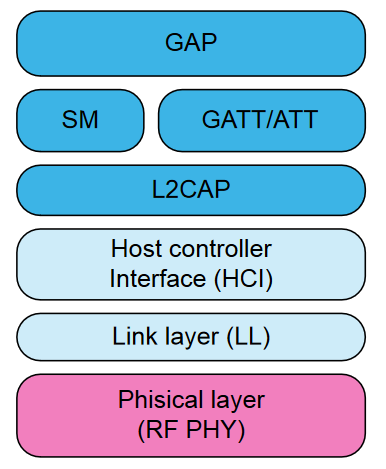
\includegraphics[scale=0.5]{imgs/ble_stack_arch}
		\caption{Arhitektura BLE stoga \cite{blemanual}}
		\label{fig:ble-stack-arch}
\end{figure}

Atributi su adresirani dijelovi informacija koji mogu sadržavati korisničke podatke ili meta-informacije o arhitekturi samih atributa. Uređaj koji prikazuje atribute naziva se poslužiteljem, a uređaj koji ih koristi naziva se klijentom. 

Atributi se sastoje od nekoliko parametara:
\begin{itemize}
	\item parametar \textit{handle}: jedinstveni 16-bitni identifikator za svaki atribut na određenom poslužitelju; svaki atribut čini adresabilnim i zajamčeno se neće mijenjati,
	\item tip: 16, 32 ili 128-bitni univerzalni jedinstveni identifikator (UUID) koji određuje vrstu podataka prisutnih u vrijednosti atributa,
	\item dopuštenja: meta-podaci koji opisuju dopuštenja za pristup ATT podacima, enkripciju i autorizaciju,
	\item vrijednost: stvarni sadržaj podataka atributa; dio atributa kojem klijent može pristupiti za čitanje i/ili pisanje.
\end{itemize}


\subsection{Upravljač}
\subsubsection{Fizički sloj}
Fizički sloj signal u radiofrekvencijskom području brzine od 1 Mbps koji prenosi informacije GFSK (\textit{Gaussian Frequency Shift Keying}) frekvencijskom modulacijom. Radi u 2,4 GHz ISM pojasu bez licence na 2400-2483,5 MHz. 
BLE sustav koristi 40 RF kanala (0-39), s razmakom od 2 MHz. Postoje dvije vrste kanala:
\begin{enumerate}
	\item Kanali za oglašavanje koji koriste tri fiksna RF kanala (37, 38 i 39) za
	\begin{enumerate}
		\item Pakete kanala za oglašavanje
		\item Pakete korištene za otkrivanje ili povezivanje
		\item Pakete korištene za odašiljanje ili skeniranje
	\end{enumerate}
	\item Podatkovni fizički kanal, koristi ostalih 37 RF kanala za dvosmjernu komunikaciju između povezanih uređaja.
\end{enumerate}

BLE je tehnologija adaptivnog skakanja frekvencije (\textit{Adaptive frequency-hopping} - AFH) koja može koristiti samo podskup svih dostupnih frekvencija kako bi se izbjegle sve frekvencije koje koriste druge neprilagodljive tehnologije. To omogućuje prelazak s lošeg kanala na poznati dobar kanal korištenjem specifičnog algoritma za skakanje frekvencije, koji određuje sljedeći dobar kanal za korištenje.

\subsubsection{Sloj veze}
Sloj veze određuje kako dva uređaja mogu koristiti signale u radiofrekvencijskom području za međusoban prijenos informacija. Također definira automat s pet stanja:
\begin{itemize}
	\item stanje pripravnosti (engl. \textit{Standby}): uređaj ne šalje niti prima pakete,
	\item oglašavanje: uređaj šalje oglase putem kanala za oglašavanje,
	\item skeniranje: uređaj traži uređaje oglašivača,
	\item pokretanje (iniciranje): uređaj pokreće vezu s uređajem oglašivača,
	\item veza: 
	\begin{itemize}
		\item uređaj  koji je inicirao komunikaciju je u ulozi \textit{master}, komunicira sa  \textit{slave} uređajem i definira vrijeme prijenosa,
		\item uređaj oglašivača je u ulozi \textit{slave}, komunicira s jednim \textit{master} uređajem.
	\end{itemize}

\end{itemize}

\begin{figure}[ht]
	\centering
	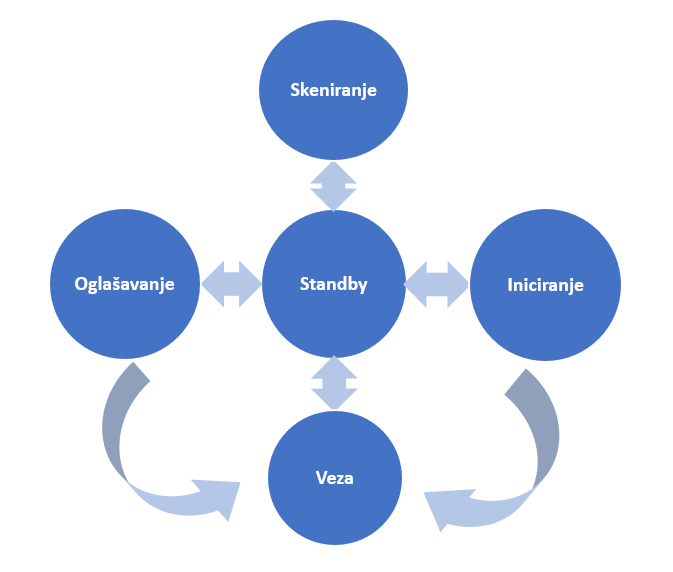
\includegraphics[]{imgs/ll_state_machine}
	\caption{Automat sloja veze \cite{blemanual}}
	\label{fig:ll-state-machine}
\end{figure}

\subsubsection{HCI}
Sučelje između domaćina i upravljača (HCI) pruža sredstvo komunikacije putem softverskog aplikacijskog programskog sučelja (\textit{Application Programming Interface} - API) ili hardverskog sučelja kao što su: SPI, UART ili USB. Dolazi iz standardnih Bluetooth specifikacija, s novim dodatnim naredbama za funkcije koje osiguravaju nisku potrošnju energije.

\subsection{Domaćin}

\subsubsection{L2CAP}
Protokol logičke veze i sloja prilagodbe (L2CAP) podržava multipleksiranje protokola više razine, operacije fragmentacije paketa i ponovnog sastavljanja, te prijenos informacija o kvaliteti usluga.

\subsubsection{SM}
BLE sloj veze (SM) podržava enkripciju i autentifikaciju korištenjem načina brojača s CBC-MAC algoritmom (kod za provjeru autentičnosti lančanih poruka) i 128-bitnu AES blok šifru (AES-CCM). Kada se enkripcija i autentifikacija koriste u vezi, 4-bajtna provjera integriteta poruke (MIC) dodaje se na jedinici podatkovnog protokola (PDU). Enkripcija se primjenjuje i na polja od PDU i MIC. Kada dva uređaja žele šifrirati podatke tijekom veze, upravitelj sigurnosti (SM) koristi postupak uparivanja. Ovaj postupak omogućuje provjeru autentičnosti dvaju uređaja razmjenom informacija o njihovu identitetu kako bi se stvorili sigurnosni ključevi koji se mogu koristiti kao osnova za pouzdani odnos ili jednu sigurnu vezu. 

\subsubsection{ATT}
Protokol atributa (ATT) definira skup metoda za otkrivanje, čitanje i pisanje atributa na drugi uređaj. Implementira \textit{peer-to-peer} protokol između poslužitelja i klijenta tipičnom zahtjev-odgovor strukturom. 


\subsubsection{GATT}
Generički atributni profil (GATT) definira okvir za korištenje ATT protokola, a koristi se za usluge, otkrivanje deskriptora, čitanje, pisanje i obavijesti. Podaci poslani putem BLE-a organizirani su ovim slojem.
U GATT kontekstu, kada su dva uređaja povezana, postoje dvije uloge uređaja:
\begin{itemize}
	\item GATT klijent: uređaj pristupa podacima na udaljenom GATT poslužitelju putem čitanja, pisanja, obavještavanja,
	\item  GATT poslužitelj: uređaj pohranjuje podatke lokalno i pruža metode pristupa podacima udaljenom GATT klijentu.
\end{itemize}

Atributi GATT poslužitelja organizirani su kao niz usluga, od kojih svaka počinje atributom deklaracije usluge koji označava njen početak. Svaka usluga grupira jednu ili više karakteristika i svaka karakteristika može uključivati nula ili više deskriptora.

\subsubsection{GAP}
Bluetooth sustav definira osnovni profil koji implementiraju svi Bluetooth uređaji. Ovaj profil naziva se generički profil pristupa (GAP), koji definira osnovne zahtjeve Bluetooth uređaja. Programska potpora mikrokontrolera implementira komunikacijsku paradigmu temeljenu na povezivanju koja pruža trajnu vezu od točke do točke (engl. \textit{point-to-point}) između dva uređaja kojom upravlja GAP sloj. Postoje četiri uloge GAP profila:
\begin{itemize}
	\item emiter (engl. \textit{broadcaster}): šalje oglase,
	\item promatrač (engl. \textit{observer}): prima oglase,
	\item periferija (engl. \textit{peripheral}): uvijek u načinu oglašavanja i u ulozi \textit{slave}, 
	\item centar (engl. \textit{central}): nikada ne šalje oglase, uvijek u \textit ulozi {master}.
\end{itemize}

Razvijena programska potpora koristi dvije od navedenih uloga, a to su periferija i centar. Periferna uloga postavljena je mikrokontroleru jer se ta uloga postavlja uređajima koji podržavaju jednu vezu i smanjenu složenost. Ovi uređaji zahtijevaju samo upravljač koji podržava ulogu \textit{slave} i koristi središnju frekvenciju upravljača za razmjenu podataka. S druge strane, centralna uloga pridružuje se uređaju koja podržava višestruke veze i pokretanje veza s perifernim uređajima. Ovi uređaji zahtijevaju upravljač koji podržava glavnu ulogu sa složenijim funkcijama, što je u ovom slučaju računalo.

\subsection{BLE komunikacija}

Na Slici \ref{fig:ble_connection_setup} prikazana je komunikacija između dva uređaja, odnosno računala i mikrokontrolera. Prema BLE specifikaciji, periferija ulazi u način oglašavanja (engl. \textit{advertisment mode}) pri pokretanju i šalje pakete oglasa u relativno dugim intervalima. Središnja jedinica ulazi u način otkrivanja (engl. \textit{discovery mode}) i šalje zahtjev za povezivanjem nakon primitka paketa oglasa od \textit{slave} uređaja. Nakon što je veza uspostavljena, obavijesti koje nose audio podatke periodično se šalju od poslužitelja do klijenta u odabranom smjeru: periferija-centar, centar-periferija ili istovremeno na oba načina. Dok je mikrokontroler u načinu oglašavanja sve do uspostave veze, računalo je u načinu otkrivanja samo kraći vremenski period te prekida sa skeniranjem dostupnih uređaja nakon zadanog vremenskog intervala.

Mikrokontroler ima ulogu \textit{slave}, dok računalo ima ulogu \textit{master}. 

\begin{figure}[ht]
	\centering
	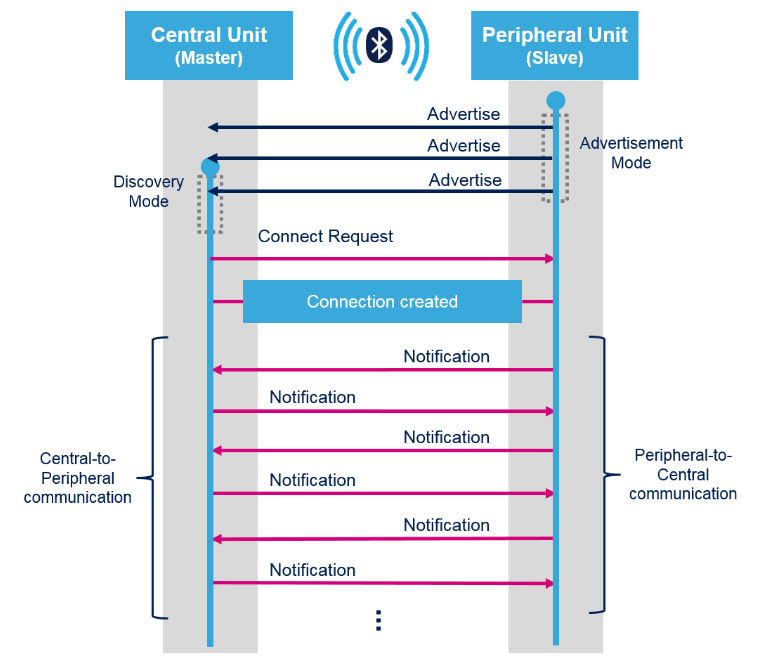
\includegraphics[scale=0.7]{imgs/ble_connection_setup}
	\caption{Uspostava BLE veze \cite{fpaudbvlink}}}
	\label{fig:ble_connection_setup}
\end{figure}


\section{MEMS mikrofon}

MEMS (\textit{Micro-Electro-Mechanical Systems}) mikrofon je elektroakustični pretvornik koji sadrži MEMS senzor i aplikacijski specifičan integrirani sklop (ASIC). MEMS mikrofoni se uglavnom temelje na elektretskim kapsulama i obično imaju ugrađena pretpojačala i analogno-digitalne pretvornike. MEMS mikrofoni su također poznati kao mikrofonski čipovi ili silikonski mikrofoni. \cite{whatismems}

Svi mikrofoni detektiraju akustične valove pomoću fleksibilne membrane, odnosno dijafragme. Membrana se pomiče pod pritiskom induciranih akustičnih valova. Danas većina MEMS mikrofona na tržištu koristi kapacitivnu tehnologiju za prikupljanje zvučnih signala. Kapacitivni MEMS mikrofoni mjere kapacitet između fleksibilne mikromembrane i fiksne stražnje ploče. Promjene tlaka zraka koje stvaraju zvučni valovi uzrokuju pomicanje membrane. Stražnja ploča je perforirana kako bi kroz nju mogao strujati zrak i dizajnirana je da ostane kruta budući da zrak prolazi kroz njezine perforacije. Kako se membrana pomiče, kapacitet se mijenja između pokretne membrane i fiksne stražnje ploče (budući da se udaljenost između njih mijenja), a ta se promjena može analizirati i zabilježiti.

Dizajn digitalnog MEMS mikrofona obično ima dodatni CMOS čip kao analogno-digitalni pretvornik. Ovi čipovi učinkovito preuzimaju pojačane analogne audio signale i pretvaraju ih u digitalne podatke. Također omogućuju lakšu integraciju digitalnih MEMS mikrofona s digitalnim proizvodima.

Najčešći format za digitalno kodiranje unutar MEMS mikrofona je modulacija trajanja impulsa (\textit{pulse-duration modulation} - PDM). PDM omogućuje komunikaciju jednom podatkovnom linijom i satom. Prijamnici PDM signala, kao i sami MEMS mikrofoni, jeftini su i lako dostupni.

\subsection{MEMS tehnologija}
Mikroelektromehanički sustavi ili MEMS je tehnologija koja se definira kao sustav minijaturiziranih mehaničkih i elektromehaničkih elemenata (tj. uređaja i struktura) koji su izrađeni mikrotvorničkim tehnikama. Fizičke dimenzije MEMS uređaja mogu varirati od znatno ispod jednog mikrometra pa sve do nekoliko milimetara. Isto tako, tipovi MEMS uređaja mogu varirati od relativno jednostavnih struktura bez pokretnih elemenata, do iznimno složenih elektromehaničkih sustava s više pokretnih elemenata pod kontrolom integrirane mikroelektronike. Jedan glavni kriterij MEMS-a je da postoje barem neki elementi koji imaju neku vrstu mehaničke funkcionalnosti bez obzira na to mogu li se ti elementi kretati ili ne.

Dok su funkcionalni elementi MEMS-a minijaturizirane strukture, senzori, aktuatori i mikroelektronika, najznačajniji elementi su mikrosenzori i mikroaktuatori. Oni su  kategorizirani kao pretvornici energije iz jednog oblika u drugi - primjerice mikrosenzor, koji obično pretvara izmjereni mehanički signal u električni.

Stvarni potencijal MEMS-a ostvaruje se kada se minijaturizirani senzori, aktuatori i strukture spoje na silicijsku podlogu zajedno s integriranim krugovima, odnosno mikroelektronikom. Dok se elektronika proizvodi pomoću sekvenci procesa integriranog kruga (npr. CMOS, bipolarni ili BICMOS procesi), mikromehaničke komponente proizvode se korištenjem kompatibilnih \textit{micromachining} procesa koji selektivno urezuju dijelove silikonske pločice ili dodaju nove strukturne slojeve kako bi formirali mehaničke i elektromehaničke uređaje. Još je kompleksnije ako se MEMS može spojiti ne samo s mikroelektronikom, već i s drugim tehnologijama kao što su fotonika, nanotehnologija itd. Ovakve konfiguracije ponekad se nazivaju heterogenom integracijom. Dok su složenije razine integracije budući trend MEMS tehnologije, sadašnja je tehnologija skromnija i obično uključuje jedan diskretni mikrosenzor, jedan diskretni mikroaktuator, jedan mikrosenzor integriran s elektronikom, mnoštvo identičnih mikrosenzora integriranih s elektronikom, jedan mikroaktuator integriran s elektronikom ili mnoštvo identičnih mikroaktuatora integriranih s elektronikom. \cite{whatismems_tech}
 

\subsection{Način rada MEMS mikrofona}

MEMS mikrofon sadrži sljedeće komponente:
\begin{itemize}
	\item MEMS pretvornik: sastoji se od membrane, perforirane ploče i kućišta,
	\item tiskana pločica (\textit{printed circuit board} - PCB): uključuje ASIC polarizacijsku jedinicu, mikrofonsko pretpojačalo i AD pretvornik,
	\item mehanički poklopac.
\end{itemize}

Zvučni valovi ulaze u MEMS mikrofon kroz poklopac i prolaze kroz perforirano kućište i ploču prije nego dođu do membrane. Valovi uzrokuju različiti zvučni tlak na membrani i razliku u tlaku između prednje i stražnje strane membrane. Ova razlika tlaka uzrokuje njeno pomicanje sukladno zvučnim valovima. Međutim, mikrofonski signal se stvara samo ako postoji naboj između vodljive membrane i Pripadajući integrirani sklop (ASIC) osigurava ovo punjenje.

Jednom napunjene, ploča i membrana mogu proizvesti napon. Budući da djeluju kao kondenzator, svaka promjena kapaciteta prouzročit će obrnuto proporcionalnu promjenu napona. Kapacitet je funkcija udaljenosti između ploče i membrane, stoga dok membrana oscilira, stvara se izmjenični napon odnosno mikrofonski signal. Ovaj napon treba pojačati da bi bio koristan kao audio signal, stoga odvojeni integrirani krug (poluvodička matrica), uključen u PCB, pojačava signal.

Ako se koristi analogni MEMS mikrofon, pojačani audio signal bi se u ovom obliku doveo na izlaz MEMS mikrofona.  Međutim, u digitalnom MEMS mikrofonu postoji dodatni proces u kojem ADC pretvara analogni signal PDM metodom prije nego što emitira digitalni audio signal.

Kao što se vidi na Slici \ref{fig:mems-mic}, stacionarna ploča je perforirana, što omogućava zraku prolaz do membrane. Na ovom je prikazu ASIC čip pričvršćen na ploču, no to nije slučaj kod svakog MEMS mikrofona. 

Stražnja je komora u ovom primjeru zatvorena, što znači da je MEMS mikrofon tlačni mikrofon - membrana je otvorena samo za zvučne valove s jedne strane, što znači da prima zvuk iz svih smjerova. Stražnja komora također djeluje kao akustični rezonator i tako pomaže pri pravilnom podešavanju mikrofona.

Također je potreban i otvor za ventilaciju kako bi stražnja komora bila pod tlakom okoline.\cite{memsdepth}

\begin{figure}[ht]
	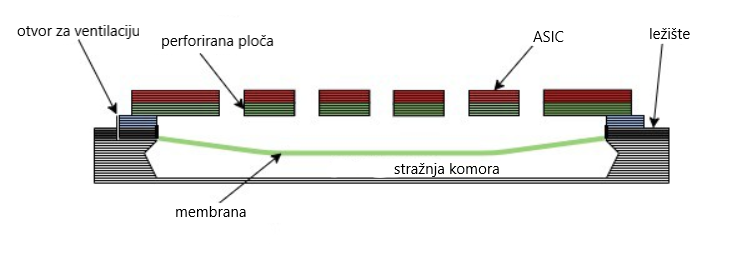
\includegraphics[width=\linewidth]{imgs/mems_mic}
	\caption{Poprečni presjek MEMS mikrofona \cite{memsdepth}}
	\label{fig:mems-mic}
\end{figure}